\section{Future Directions}\label{sec:future}


\begin{figure}[ht]
  \centering
  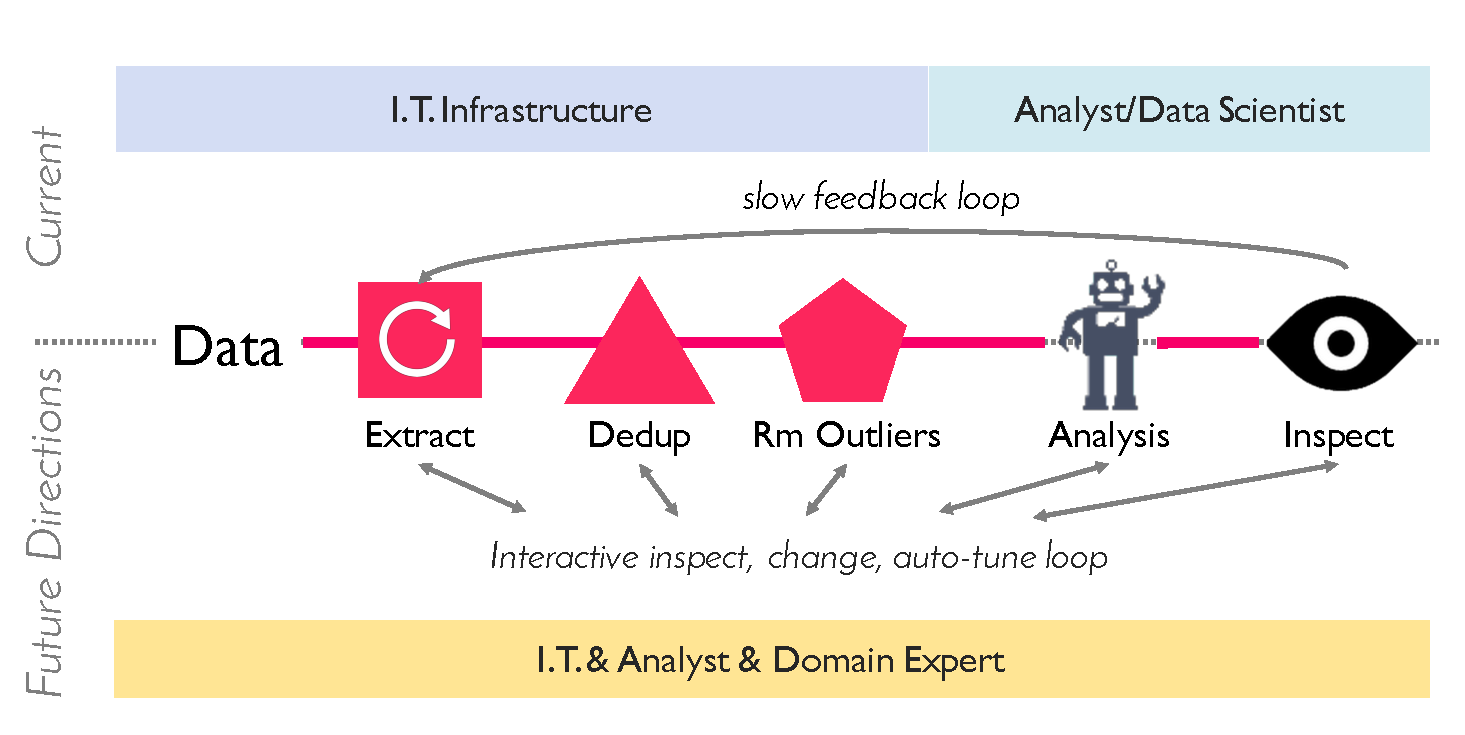
\includegraphics[width=.95\columnwidth]{datafigs/arch}
  \caption{Current and proposed iterative feedback loop for data cleaning.  
  The top shows the current slow feedback loop, where the data cleaning (magenta) and analysis (robot) steps are split between I.T. and data scientists, and feedback is obtained from the data scientists. 
  The bottom shows the potential unified approach, where the cleaning can be inspected or modified by any user at any step throughout the pipeline.  This can happen through manual changes or auto-tuned optimizations.
  }
  \label{f:arch}
\end{figure}

Our initial survey results highlighted several bottlenecks that add friction to the data cleaning and analysis process.
The primary finding reiterates the observation that data cleaning is highly contextual~--~users intimately familiar with the downstream applications are needed to direct the data cleaning process.  In other words, these domain experts are the most important ``humans in the data cleaning loop''.  

In practice, however, we found that the data cleaning process is commonly split across multiple organizational units: the IT department performs data cleaning, and sends the processed data to application developers and data scientists, who in turn perform additional data transformation and analysis (top of Figure~\ref{f:arch}).  This separation inhibits the ability to experiment and test different cleaning procedures and tune their parameters---feedback about the data cleaning process is often delayed until the downstream application developer (e.g., visually) inspects the application results.  We believe that these limitations need not exist, and envision a highly interactive data cleaning and analysis process, wherein infrastructure engineers, data analysts and domain experts can design, evaluate, and modify (with automated support) any stage of the data cleaning workflow (bottom of Figure~\ref{f:arch}). To this end, we present a series of technical challenges spanning HCI, statistics, and data management that must be overcome in order to support a truly interactive data cleaning system.

% As highlighted in the top half of Figure~\ref{f:arch}, changes to the cleaning process occur based on observations made at the end of the analysis pipeline.  

\vspace{0.5em}
\noindent\textbf{Developing High-level Language for Domain Experts:} Data cleaning is an involved process that involves extraction, schema/ontology matching, value imputation, de-duplication, and other processes.
In addition, each of these operations encapsulates dozens of specialized algorithms such as machine learning, clustering, or rule-based procedures.
It is both difficult for domain experts to navigate through the zoo of options, and easy for those implementing data cleaning operations to become married to a specific algorithmic choice.
In addition, these parties must interact, and it is important to facilitate the coordination between the two.
There is a need for a high level language for domain experts to describe the data cleaning goals at a logical level (e.g., providing de-duplication examples, descriptions of outliers) that also enables physical implementation choices to be guided by either automated tools or the technical experts that are tasked with implementing data cleaning at scale~\cite{DBLP:conf/sigmod/Galhardas00,wisteria}. 

\vspace{0.5em}
\noindent\textbf{Usability and Interactivity:} The need to focus on usability and visual interaction has been reiterated across many domains:  Wrangler~\cite{kandel2011wrangler} (commercialized as Trifacta~\cite{trifacta}) enables domain experts to perform complex text extraction tasks at scale, and  Polaris~\cite{stolte2002polaris} (commercialized as Tableau~\cite{tableau}) helps business analysts perform data-cube analysis through a visual interface. These systems place emphasis on the end-to-end process by reducing bottlenecks that stem from human interaction and decision making.    We must similarly lift a high level cleaning language into the interactive domain~\cite{heer2015predictive} in order to tighten the feedback loop between the user and cleaning process.

% Often times the domain experts are not techincal experts\footnote{Although our user study population is biased towards technical users, other studies~\cite{kandel2012} have shown that data analysts are often non-technical domain experts.}, and there is a need to map the high-level language into the visual interactive domain.  We have seen success from intergrating a domain specific language and visual interactions  in specialized data cleaning domains such as text extraction~\cite{kandel2011wrangler}.  Similarly agreementmaker work.
% 
% long pipeline from cleaning and output, so insert inspection.  
\vspace{0.5em}
\noindent\textbf{Application-oriented Cleaning:}  A recurring theme amongst our survey participants was the observation that data cleaning is driven by the needs of the downstream application.  We found surprisingly little evidence of data cleaning as a discrete and isolated process. Systems such as SampleClean~\cite{DBLP:journals/debu/KrishnanWFGKM015} and ActiveClean~\cite{activecleanarxiv} have already shown the potential for leveraging application knowledge to reduce data cleaning costs by an order of magnitude or more compared to application agnostic approaches.  However these systems have been tailored to specialized use cases (individual aggregation queries and convex models, respectively), and support for other more complex operations as well as multi-stage sequences of analyses is needed.

\vspace{0.5em}
\noindent\textbf{Human-Computer Symbiosis:}   Some participants described tweaking cleaning operations and running the downstream analysis in order to visually inspect the results.  However, this form of manual configuration and parameter tuning does not make the best use of the domain expert's resources.   There is potential to introduce automation, and we have already seen examples of this.  For instance, active learning is used as part of crowd-sourced label acquisition~\cite{gokhale2014corleone,DBLP:journals/pvldb/HaasW0F15} to optimize an operation such as de-duplication;  Wrangler automatically generates string extraction rules so that the user only needs to pick from a set of options; and TuPAQ~\cite{sparks2015automating} performs automatic hyper-parameter tuning for machine learning models.   There is similar opportunity to identify additional data cleaning operations that can be automatically tuned, as well as to propose modifications to the sequence of operations itself~\cite{wisteria}.  Ultimately, our goal should be to let experts do what they do best, while machines do the rest.

\vspace{0.5em}
\noindent\textbf{Testing and Debugging:} In order to develop automated optimization and tuning procedures, there must be a metric to optimize.  This can be quite challenging---one common measure of data cleaning effectiveness among survey participants was simply whether or not the downstream process compiled and ran!
This clearly falls short of the standards needed for sophisticated automation, and methods for introducing metrics throughout the cleaning and analysis process are needed.
For example, one might use performance on gold examples of known clean data to evaluate a cleaning operator.
Such data could be acquired up front, or adaptively collected from the analyst herself or crowd workers throughout the cleaning process.

As the data analyst inspects different parts of the cleaning process, it will be increasingly important to provide tools to summarize and explain~\cite{DBLP:journals/pvldb/0002M13,DBLP:conf/sigmod/ChalamallaIOP14,wang2016qfix} the intermediate results in a way to goes beyond print statement outputs or row data entries.

In addition, to accelerate data cleaning research, there is a need for a cleaning benchmark analogous to industry standard transaction and analytical data processing benchmarks.
Existing systems are often evaluated on synthetically generated errors that are may not reflect reality or on application-specific errors that are too specialized to serve as a standard benchmark across systems.

%Such a benchmark needs to support cases when there is and is not a ground truth dataset.
\vspace{0.5em}
\noindent\textbf{Combating Over-fitting:}
Despite their importance, data cleaning procedures are often under-reported
when presenting the results of data analysis. This is problematic since the data
cleaning operations have a potential to introduce analyst biases,
i.e., favoring a certain outcomes, into the analysis process.
This sentiment is corroborated by our survey results and the results of Kandel et al.~\cite{kandel2012}.
In a sense, this problem is analogous to statistical over-fitting, where cleaning decisions based on strong assumptions over a small sample of data (or a specialized analysis) may not apply to future evolutions of the application.
An important challenge is designing data cleaning tools that: (1) allow analysts to communicate assumptions (e.g., which records have been removed) when presenting results, (2) automatically determine when an assumption is risky (e.g., correlates with the tested hypothesis), and (3) manages a ``paper trail'' of data transformations.


\section{Conclusion}
We have presented initial results from a study of industry users of data analysis software that confirms the recent shift in data cleaning processes towards iterative workflows.
Our survey results highlight the issues that frustrate current workflows, and motivate our proposal of the research challenges central to the design of unified systems that can alleviate these issues.
In summary, though the data cleaning community is in the early days of highly interactive data cleaning and preparation, there are clear opportunities for systems that facilitate and automate rapid human-in-the-loop interactivity.

\vspace{0.5em}
\small
\textbf{This research is supported in part by NSF CISE Expeditions Award CCF-1139158, DOE Award SN10040 DE-SC0012463, and DARPA XData Award FA8750-12-2-0331, and gifts from Amazon Web Services, Google, IBM, SAP, The Thomas and Stacey Siebel Foundation, Apple Inc., Arimo, Blue Goji, Bosch, Cisco, Cray, Cloudera, Ericsson, Facebook, Fujitsu, HP, Huawei, Intel, Microsoft, Pivotal, Samsung, Schlumberger, Splunk, State Farm and VMware.}

